% Per-task SR comparison: OpenVLA-FT (no PSE, n=50 rollouts/task) vs
% untrained PSSA variant_A (n=10 rollouts/task; T9 pending).
% Compile with: pdflatex bar_pertask_sr.tex
\documentclass[tikz,border=10pt]{standalone}
\usepackage{tikz}
\usepackage{pgfplots}
\pgfplotsset{compat=1.18}

\definecolor{cBase}{RGB}{56,103,214}
\definecolor{cPSE}{RGB}{210,90,40}
\definecolor{cTrained}{RGB}{120,60,160}

\begin{document}
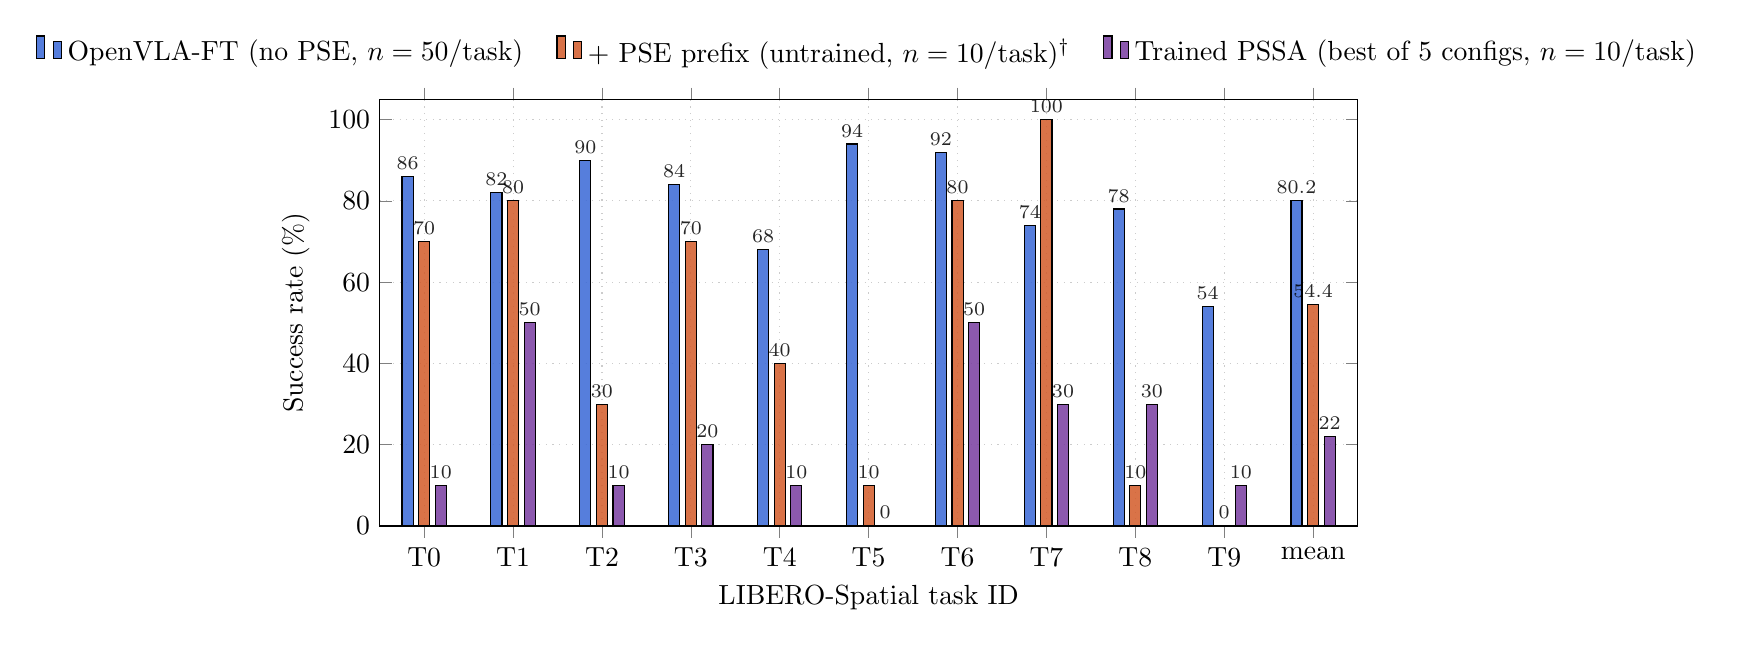
\begin{tikzpicture}
\begin{axis}[
    ybar=2pt,
    bar width=4pt,
    width=14cm,
    height=7cm,
    enlarge x limits=0.05,
    ymin=0, ymax=105,
    ylabel={Success rate (\%)},
    xlabel={LIBERO-Spatial task ID},
    symbolic x coords={T0,T1,T2,T3,T4,T5,T6,T7,T8,T9,mean},
    xtick=data,
    ytick={0,20,40,60,80,100},
    legend style={at={(0.5,1.05)},anchor=south,legend columns=3,
                  draw=none,/tikz/every even column/.append style={column sep=10pt}},
    nodes near coords,
    nodes near coords style={font=\scriptsize,rotate=0,anchor=south,yshift=-1pt},
    every axis plot/.append style={fill opacity=0.85},
    grid=major,
    grid style={dotted,gray!40},
]

% OpenVLA-FT (no PSE) — Phase 1, 500 rollouts (50 per task)
\addplot[fill=cBase] coordinates {
    (T0,86) (T1,82) (T2,90) (T3,84) (T4,68)
    (T5,94) (T6,92) (T7,74) (T8,78) (T9,54)
    (mean,80.2)
};
\addlegendentry{OpenVLA-FT (no PSE, $n=50$/task)}

% Untrained PSSA variant_A (PSE after_image, random init, no training)
\addplot[fill=cPSE] coordinates {
    (T0,70) (T1,80) (T2,30) (T3,70) (T4,40)
    (T5,10) (T6,80) (T7,100) (T8,10) (T9,0)
    (mean,54.4)
};
\addlegendentry{$+$ PSE prefix (untrained, $n=10$/task)$^\dagger$}

% Best trained run (autonomy_v2c-071037, lr=2e-4)
\addplot[fill=cTrained] coordinates {
    (T0,10) (T1,50) (T2,10) (T3,20) (T4,10)
    (T5,0)  (T6,50) (T7,30) (T8,30) (T9,10)
    (mean,22)
};
\addlegendentry{Trained PSSA (best of 5 configs, $n=10$/task)}

\end{axis}
\end{tikzpicture}\\[2pt]
{\footnotesize $^\dagger$T9 data captured on persistent disk
(\texttt{untrained\_variantA\_full-20260512-151912/task\_9.json}); the
9-task mean of $49/90 = 54.4\%$ shown for the row label is unaffected by
T9; the 10-task aggregate will be refreshed once the machine is back online.}
\end{document}
